\documentclass[11pt]{article}
\usepackage{fullpage,fourier,euler,amsmath,graphicx,xspace,amssymb}
\usepackage{epigraph,wrapfig}
\usepackage{listings,color,url,hyperref}
\usepackage[x11names]{xcolor}

% https://www.scientificamerican.com/article/the-tower-of-hanoi/

\title{Assignment 4 \\ The Tower of Brahma}
\author{Prof. Darrell Long \\
CSE 13S -- Fall 2019}
\date{Due: October 27th at 11:59\,pm}

\usepackage{fancyhdr}
\pagestyle{fancy}
\fancyhf{}

\fancypagestyle{plain}{%
  \fancyhf{}
  \renewcommand{\headrulewidth}{0pt}
  \renewcommand{\footrulewidth}{0pt}
  \lfoot{\textcopyright{} 2021 Darrell Long}
  \rfoot{\thepage}
}

\pagestyle{plain}

\definecolor{codegreen}{rgb}{0,0.5,0}
\definecolor{codegray}{rgb}{0.5,0.5,0.5}
\definecolor{codepurple}{rgb}{0.58,0,0.82}

\lstloadlanguages{C,make,python,fortran}

\lstdefinestyle{c99}{
    morekeywords={bool, uint8_t, uint16_t, uint32_t, uint64_t, int8_t, int16_t, int32_t, int64_t},
    commentstyle=\color{codegreen},
    keywordstyle=\color{magenta},
    numberstyle=\tiny\color{codegray},
    identifierstyle=\color{blue},
    stringstyle=\color{codepurple},
    basicstyle=\ttfamily,
    breakatwhitespace=false,
    breaklines=true,
    captionpos=b,
    keepspaces=true,
    numbers=left,
    numbersep=5pt,
    showspaces=false,
    showstringspaces=false,
    showtabs=false,
    tabsize=4
}

\lstset{language=C, style=c99}

\begin{document}\maketitle

\section{Introduction}
\epigraphwidth=0.8\textwidth
\epigraph{\emph{Dans ses voyages pour la publication des \'ecrits de
l'illustre \emph{Fer-Fer-Tam-Tam}, dans le grand temple de B\'enar\`es,
au-dessous du d\^ome qui marque le centre du monde, trois aiguilles
de diamant, plant\'ees dans une dalle d'airain, hautes d'une coud\'ee
et grosses comme le corps d'une abeille. Sur une de ces aiguilles,
Dieu enfila au commencement des si\`ecles, 64 disques d'or pur, le
plus large reposant sur l'airain, et les autres, de plus en plus
\'etroits, superpos\'es jusqu'au sommet. C'est la tour sacr\'ee du Brahm\^a.
Nuit et jour, les pr\^etres se succ\`edent sur les marches de l'autel,
occup\'es \`a transporter la tour de la premi\`ere aiguille sur la
troisi\`eme, sans s'\'ecarter des r\`egles fixes que nous venons d'indiquer,
et qui ont \'et\'e imposées par Brahm\^a. Quand tout sera fini, la tour
et les brahmes tomberont, et ce sera la fin des mondes!}}{---N.\ Claus de
Siam, 1883}


\begin{wrapfigure}{r}{0.25\textwidth}
\centering
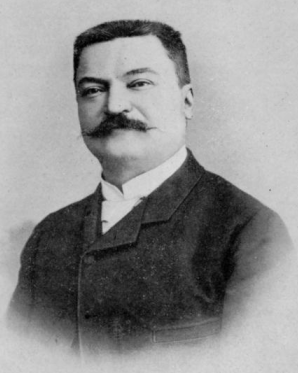
\includegraphics[width=0.2\textwidth]{Elucas_1}
\caption{Edouard Lucas}
\end{wrapfigure}
In the great temple of Benares, below the dome
which marks the center of the world, three diamond needles are planted
on a slab of brass, one cubit high and as large as the body of a
bee. On one of these needles, God put forth at the beginning of the
centuries, 64 disks of pure gold, the largest resting on the brass,
and the others, more and more narrow, superimposed to the summit.
It is the sacred tower of Brahma. Night and day, the priests succeed
one another on the steps of the altar, busy carrying the tower of
the first needle on the third, without departing from the fixed
rules which we have just indicated, and which have been imposed by
Brahma. When all is over, the tower and the Brahmins will fall,
and it will be the end of the world!

This is also known as the ``End of the World Puzzle'' or ``The Lucas Tower,'' named after the French mathematician Eduoard Lucas in 1883. The puzzle is now famous with the name ``The Tower of Hanoi.''

Like the legend establishes, the Tower of Hanoi consists of three
pegs. Initially, the player is a given a stack of discs, each one
progressively larger than the next. The object of the game is to
move all the disks to another peg, only moving one disk at a time
and never placing a larger disk on top of a smaller disk.

\begin{figure}[tb]
\begin{centering}
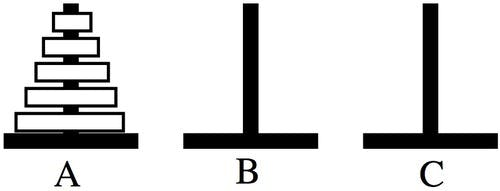
\includegraphics[width=0.75\textwidth]{towers}
\caption{Towers of Hanoi.}\label{tower}
\end{centering}
\end{figure}


%%%%%%%%%%%%%%%%%%%%%%%%%%%%%%%%%%%%%%%%%%%%%%%%%%%%%%%%

\section{The Problem}
The game is rather simple when there are only two to three disks. However, as the number of disks increase so does the difficulty and amount of steps to complete the game.

The objective of the game is simple -- move all the disks from column A to column B. However there are two simple rules:

\begin{enumerate}
  \item Only one disk can be moved at a time.
  \item No larger disk can be placed on top of a smaller disk.
\end{enumerate}

To get an understanding of how the game works, we recommend playing around with the disks first:
\url{https://www.mathsisfun.com/games/towerofhanoi.html}.
If you think it throughly, you will see that there is a pattern. You are not searching for a solution; you are simply following the same steps over and over.

You will implement this puzzle in two ways, with recursion and using a stack.

\subsection{Recursion}
Recursion is when a function calls itself. It is useful in solving
problems that can be broken down into smaller sub-problems.
Mathematicians call this puzzle a recursive procedure. To solve the
puzzle with more disks, you start out with the solution for a smaller
number of disks.

The fundamentals of recursion include a base case and the recursive
call. The base case is the terminating case that helps you break
out of the recursive function, otherwise your program would go on
indefinitely.

Why do you need recursion? You do not need it really, but you do
need to track the disks. If you are na\"ive then you may get caught
up making the same moves over and over again. \textcolor{red}{A
good question to ask yourself is: How do you prevent making the
same wrong choice twice?}


\subsection{Stack}
A stack is a linear data structure that follows either a LIFO
(last-in, first-out) or FILO (first-in, last-out) order.  Stacks
play a role in a lot of real-life examples. One example being the
undo and redo commands in document editors. How does Microsoft Word
remember what sentence we're referring to when we press CTRL\texttt{+}Z?
By using a stack.

How can you use a stack to implement Towers of Hanoi? If you're familiar with this game or if you've played around with the game, you'll notice that each peg is a physical stack. You will need to implement the stack data structure for this assignment. To implement Towers of Hanoi, you will treat each peg as a stack.

How many stacks do you need? You could use one, and simply mimic the recursion,
but it makes sense to treat each peg as a stack.

How many moves does it take?
$x_n = 2 x_{n-1} + 1$ with $x_0 = 0$ (this base case should be obvious)
which means that $x_n = 2^n - 1$, again a recursion
that you will learn how to solve in CSE 16.

\begin{lstlisting}[title=stack.h]
// stack.h - Contains the function declarations for the Stack ADT.

#ifndef __STACK_H__
#define __STACK_H__

#include <inttypes.h>
#include <stdbool.h>

//
// Struct definition for a Stack.
//
// name:       The Stack's single-character identifier.
// top:        Keeps track of the top of the Stack.
// capacity:   The maximum number of items a Stack can hold.
// items:      The array to store Stack items in.
//
typedef struct Stack {
    char name;
    int top;
    int capacity;
    int *items;
} Stack;

//
// Constructor for a new Stack.
//
// capacity:   The maximum number of items the Stack can hold.
// name:       The Stack's single-character identifier.
//
Stack *stack_create(int capacity, char name);

//
// Destructor for a Stack.
//
// s:  The Stack to free allocated memory for.
void stack_delete(Stack *s);

//
// Pops an item off a Stack if it isn't empty.
//
// s:  The Stack to pop an item off of.
//
int stack_pop(Stack *s);

//
// Pushes an item into a Stack if it isn't full.
//
// s:  The Stack to push an item into.
//
void stack_push(Stack *s, int item);

//
// Returns true if a Stack is empty and false otherwise.
//
// s:  The Stack to query about being empty.
bool stack_empty(Stack *s);

# endif
\end{lstlisting}


%%%%%%%%%%%%%%%%%%%%%%%%%%%%%%%%%%%%%%%%%%%%%%%%%%%%%%%%

\section{Your Task}
\begin{itemize}
  \item You must use \texttt{getopt} to parse command line arguments for the
      following options:
      \begin{enumerate}
          \item ``\texttt{-n x}'' : sets the number of disks to \texttt{x} (x is
              defaulted to 5 if this option isn't supplied).
        \item ``\texttt{-s}'' : print out the moves performed using the stack
            implementation.
        \item ``\texttt{-r}'' : print out the moves performed using the
            recursive implementation.
      \end{enumerate}

  \item Your program must print the number of moves used. Refer to the included output example.

  % \item Your program must also calculate the minimum amount of moves required for \texttt{x} amount of disks and print that number out to the command line.

  \item The output of your program must follow the format of the examples provided below. For example, for printing out the disk moves the output should be: ``Move disk Z from peg X to peg Y''
\end{itemize}

\begin{lstlisting}
TheMachine:tower darrell$ ./tower -s -r
================================
----------   STACKS   ----------
================================
Move disk 1 from peg A to peg B
Move disk 2 from peg A to peg C
Move disk 1 from peg B to peg C
Move disk 3 from peg A to peg B
Move disk 1 from peg C to peg A
Move disk 2 from peg C to peg B
Move disk 1 from peg A to peg B
Move disk 4 from peg A to peg C
Move disk 1 from peg B to peg C
Move disk 2 from peg B to peg A
Move disk 1 from peg C to peg A
Move disk 3 from peg B to peg C
Move disk 1 from peg A to peg B
Move disk 2 from peg A to peg C
Move disk 1 from peg B to peg C
Move disk 5 from peg A to peg B
Move disk 1 from peg C to peg A
Move disk 2 from peg C to peg B
Move disk 1 from peg A to peg B
Move disk 3 from peg C to peg A
Move disk 1 from peg B to peg C
Move disk 2 from peg B to peg A
Move disk 1 from peg C to peg A
Move disk 4 from peg C to peg B
Move disk 1 from peg A to peg B
Move disk 2 from peg A to peg C
Move disk 1 from peg B to peg C
Move disk 3 from peg A to peg B
Move disk 1 from peg C to peg A
Move disk 2 from peg C to peg B
Move disk 1 from peg A to peg B

Number of moves: 31

================================
--------   RECURSION   ---------
================================
Move disk 1 from peg A to peg B
Move disk 2 from peg A to peg C
Move disk 1 from peg B to peg C
Move disk 3 from peg A to peg B
Move disk 1 from peg C to peg A
Move disk 2 from peg C to peg B
Move disk 1 from peg A to peg B
Move disk 4 from peg A to peg C
Move disk 1 from peg B to peg C
Move disk 2 from peg B to peg A
Move disk 1 from peg C to peg A
Move disk 3 from peg B to peg C
Move disk 1 from peg A to peg B
Move disk 2 from peg A to peg C
Move disk 1 from peg B to peg C
Move disk 5 from peg A to peg B
Move disk 1 from peg C to peg A
Move disk 2 from peg C to peg B
Move disk 1 from peg A to peg B
Move disk 3 from peg C to peg A
Move disk 1 from peg B to peg C
Move disk 2 from peg B to peg A
Move disk 1 from peg C to peg A
Move disk 4 from peg C to peg B
Move disk 1 from peg A to peg B
Move disk 2 from peg A to peg C
Move disk 1 from peg B to peg C
Move disk 3 from peg A to peg B
Move disk 1 from peg C to peg A
Move disk 2 from peg C to peg B
Move disk 1 from peg A to peg B

Number of moves: 31

\end{lstlisting}

\begin{lstlisting}
TheMachine:tower darrell$ ./tower -s -n 3
================================
----------   STACKS   ----------
================================
Move disk 1 from peg A to peg B
Move disk 2 from peg A to peg C
Move disk 1 from peg B to peg C
Move disk 3 from peg A to peg B
Move disk 1 from peg C to peg A
Move disk 2 from peg C to peg B
Move disk 1 from peg A to peg B

Number of moves: 7
\end{lstlisting}

%%%%%%%%%%%%%%%%%%%%%%%%%%%%%%%%%%%%%%%%%%%%%%%%%%%%%%%%
\section{Deliverables}

\noindent You will need to turn in:

\begin{enumerate}
  \item \texttt{tower.c}: The source file which contains your program.

  \item \texttt{Makefile}: This is a file that will allow the grader to type \texttt{make} to compile your program. Typing \texttt{make} must build your program and \texttt{./tower} alone as well as with flags must run your program.
  \begin{itemize}
    \item \texttt{CFLAGS=-Wall -Wextra -Werror -Wpedantic} must be included.
    \item \texttt{CC=clang} must be specified.
    \item \texttt{make clean} must remove all files that are compiler generated.
    \item \texttt{make} should build your program, as should \texttt{make all}.
\item As for every assignment from now on, \texttt{make infer} should run
\texttt{infer}. You \emph{must} fix any errors that \texttt{infer} finds, or
explain why \texttt{infer} is incorrect.
  \end{itemize}

  \item \texttt{stack.c and stack.h}: We will provide you with the header file, however it is your job to implement the functions. These two files will contain your stack implementation.

  \item \texttt{README.md}: This can either be in \emph{markdown} or PDF. This must describe how to use your program and \texttt{Makefile}.

  \item \texttt{DESIGN.md}: This \emph{must} be in \emph{markdown}. The design document
  should describe your design for your program with enough detail
  that a sufficiently knowledgeable programmer would be able to
  replicate your implementation. This does not mean copying your
  entire program in verbatim. You should instead describe how your
  program works with supporting pseudo-code.

  \item \texttt{WRITEUP.pdf}: This \emph{must} be a PDF. Your WRITEUP should be a discussion of the results for your
  experiments. For this assignment, comment on the comparable complexity of both solutions.

\end{enumerate}

%%%%%%%%%%%%%%%%%%%%%%%%%%%%%%%%%%%%%%%%%%%%%%%%%%%%%%%%

\section{Submission}

To submit your assignment, refer back to \texttt{assignment0} for
the steps on how to submit your assignment through \texttt{git}.
Remember: \emph{add, commit,} and \emph{push}!

\textcolor{red}{Your assignment is turned in \emph{only} after you
have pushed.  If you forget to push, you have not turned in your
assignment and you will get a \emph{zero}. ``I forgot to push'' is
not a valid excuse. It is \emph{highly} recommended to commit and
push your changes \emph{often}.}

\end{document}
